\chapter{Machine Learning approach} \label{chap:system_archi}
This chapter introduces the industry standard used in any machine learning project followed by elaborating the phases and mapping them to a machine learning project. This chapter also introduces the different modelling approach used given the theme of this work and introduce to the different experiments conducted.

\section{Process Methodology} \label{sect:Kdd}
The advancement in the processing huge amounts of data led to the transition from the manual process of analysing considerable databases to a more sophisticated and automated one. Such processes are completed by algorithms which can extract relationships from a massive amount of data. This development led to the widespread adoption of Machine Learning and Data Mining algorithms in applications across different industries. Some of the examples of such applications are  Image recognition, Natural Language Processing, Sentiment Analysis, to name few. To implement such a novel application in industry, a standardised method is required which provides the set of guidelines for implementing such projects on an enterprise level. For software development practises, frameworks like Software Development Life Cycle(SDLC), Waterfall model, Agile are widely used, which makes the software development process efficient. Similarly for Machine Learning and Data Mining related projects, process models such as CRoss Industry Standard Process for Data Mining (CRISP-DM), Knowledge Discovery in Databases (KDD), and Sample Explore Modify Model and Assess (SEMMA) are standard. For this project work, the KDD process model is referred to, which is explained in this section and map its defined phases to the project phases. \\ 
\par


\begin{figure}
    \centering
    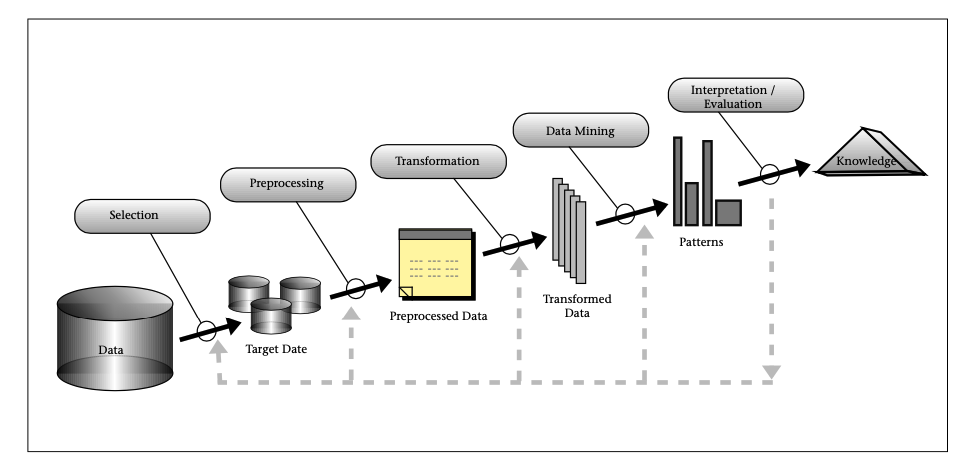
\includegraphics[scale=0.5]{chapters/figures/CRISP-DM.png}
    \caption{Different phases of KDD process model. \\ 
    Source: In the \textcite[41]{fayyad1996data}}
    \label{fig:CRISP_DM}
\end{figure}

A standard methodology helps the stakeholders in understanding the critical issues related to the data mining process. Additionally, it also introduces a structure to the project and benefits the analysts and engineers by referring to the set of instructions. KDD process model more emphasises explicitly on the entire process of knowledge from large data sources \autocite[39]{fayyad1996data}. The KDD process methodology primarily identifies the essential tasks and categorise them into five main steps, namely: Selection, Pre-processing, Transformation, Data Mining, Evaluation and Interpretation \autocite[42]{fayyad1996data}. The phases defined are interlinked where the output of a phase acts as an input to another phase. Some phase might often require iteration on the continuous improvement; hence they are repeated. Although the sequential nature of the process is indicated in the KDD process (see \ref{fig:CRISP_DM}), it is not mandatory to perform a particular activity in that sequence. The detailed explanation of the activities carried out in each phase are described as follows:


\begin{itemize}
    \item \textit{Selection}: \\
The initial step in any project is to understand the existing problem scenario, followed by gathering the necessary information to address the problem. Once achieved the \textit{Selection} step is more focused on discovering different sources of information and, selecting appropriate data from which it expects to discover meaningful patterns.  More specific activities performed in this step are identifying appropriate data source, variables associated with the main business problem. In this work, the company-wide database examined for information regarding the products, consumers. Furthermore, the transactional database if used to get the transactions completed in the year 2017 and 2019.  This step results in the target data, which supports the activities in the next step.

    \item \textit{Pre-processing}: \\
    Once the data source has is identified, the next step is pre-processing the data set obtained. It involves removing unnecessary information, replacing missing values, removing duplicate values, and other data formatting activities to generate pre-processed data. 
    
    \item \textit{Transformation}:\\
     Most of the time, the raw transactional data is in relational format i.e. in tabular format. Thus in order to make the data useful, it needs to be transformed into an appropriate format. The format of the data depends on the underlying machine learning algorithm used. Furthermore, machine learning algorithms require data for the features in numeric format. Thus, data transformation techniques, such as categorical encoding, scaling, etc., are performed. Additionally, if required, the pre-processed data is transformed to lower dimensions from its raw form. Dimensionality reduction techniques help identify the features in the data which are representative enough of the data. 
    \item \textit{Data Mining}:\\
    This step involves identifying the pattern within the data by creating a model using machine learning algorithms. Depending on the objective of the entire process, different types of algorithms used individually or in combination to form an ensemble in this step.  
    \item \textit{Evaluation and Interpretation}:\\
    The evaluation of the model helps in understanding the effectiveness in identifying the pattern given the objective. Different metrics used to measure the performance of the model created. The performance of the model can be further improved by experimenting and identifying an appropriate set of parameters, also known as hyper-parameter for the algorithm.  
\end{itemize}


\section{Dataset and Pre-Processing} \label{sect:thefirst}
The process of identifying appropriate data sources which represent the business problem is crucial for the entire project. Any inconsistency, can lead to undesirable results resulting in considerable amount of resources. Therefore keeping in mind the business problem, the data-set for developing recommender system is carefully selected. This stage can be related to the \textit{Selection} phase of the KDD model as discussed above. \\ \Par

\begin{table}
\begin{tabular}{ |m{0.5cm}| m{3cm} | m{8cm}| m{2cm} | } 
\hline 
No. & Feature & Feature Description & Datatype \\ 
\hline \hline
1 & user{\_}id
 & Represents the unique identifier assigned to each dealer (in recommender system terminology it represents the user). It is one of the key feature in the the modelling process. & integer \\ 
\hline
2 & item{\_}id & Represents the unique identifier assigned to each active item present in the product catalogue. Along with user{\_}id, item{\_}id is another primary feature. & integer. \\
\hline
3 & item description & Provides and description of the item. & string \\
\hline
4 & artikel{\_}group & Represents the article group to which it the item belongs.This feature represents the contextual information and be used by converting it into a variable of type category. & string \\
\hline
5 & brand & Represents the brand under which the item is sold. Similar to the artike{\_}group feature, this feature can also be converted into a category group. This feature represents additional contextual information about the item. & string \\
\hline
6 & order{\_}id & The unique order{\_}id assigned for each transaction completed. Apart from uniquely identifying each transaction, this feature has no significant contribution to the modelling process and hence will be ignored from further processing process. & integer \\
\hline
7 & user{\_}name & The unique name assigned each of the dealer. Since a unique identifier user{\_}id is sufficient, this feature can be ignored from further processing. & string \\ 
\hline
8 & quantity & Represents the quantity of the items purchased in a order. & integer \\
\hline
9 & purchase{\_}date & Denotes the date on which a particular purchase was made. Additional contextual features like, month, year can be extracted denoting the time related patterns.  & string (YYYY-MM-DD) format. \\
\hline
10 & plz & Denotes the postal code of the dealer where he is located. This feature can be considered as context feature as it can help in gathering location related information.  & integer \\
\hline
10 & season & Denotes the season in which the purchase was made. This feature is derived from the feature \textit{purchase{\_}date}. Observing this feature over the period can be helpful in identifying seasonality pattern. It takes binary value i.e. 1= Summer,0= Winter. & integer (binary format) \\
 \hline
\end{tabular}
\label{table:features}
\caption{Overview of the features in the data-set \\
Source: Own Investigation}
\end{table}

Since there is no online web-shop designed at this moment at RTI Sports, the most consistent source of information which used is the transactional database. This database consists of different transactions that completed in the past, along with additional information. For this study, transactional data for the past three years, i.e. 2017,2018,2019 is considered. Additionally, information about the actual items and the dealers ( which represent the items and users respectively in recommender system terminology) extended for the analysis. Table \ref{table:features} gives an overview of the columns present in the selected data-set. The table describes the importance of each feature and the datatype which it represents. \\ \par

The 2nd step in the KDD process is to pre-process the selected data, which will result in clean data-set. One such example is to fill up missing values. In the given data-set, there were some missing values for the feature \textit{PLZ}, which were replaced with its appropriate value. Additionally, there were some items and item group which ceased from the production. Such items and item groups were identified, and transactions for those items were removed from further analysis. The extracted data, along with the information about the items and the users is pre-processed to identify and remove any unwanted or anomalous information. On completion, initial analysis of the data-set is performed, which allows us to gain some intuition about the data. This process is also known as Exploratory Data Analysis (EDA). This process involves showing the characteristics of the data in a visual format such as plots. Based on the initial observation, in the entire data-set, there are many users who have just bought a handful of items in the given timeline. Hence, in order to create a meaningful test and train set, only those users who have purchased more than five items in the past are considered for the modelling process. After filtering out the users, the following statistics about the users and the articles obtained are shown in Table \ref{tab:data}.\\ 
\Par

\begin{table}[t]
\centering
\begin{tabular}{|l|c|}
\hline
Feature & Unique Count\\
\hline\hline
user{\_}id & 2528\\
\hline
item{\_}id  &  1496\\
\hline
unique orders & 138985  \\
\hline
user-item interactions  & 694958\\
\hline
item{\_}group & 68 \\ 
\hline
brand & 8\\ 
\hline
\end{tabular}
\caption{Summary of the selected data-set \\
Source: Own Investigation}
\label{tab:data}
\end{table}


The initial analysis also reveals, that there are very few items that are popular, whereas the other items are less popular among the customers. This scenario is also known as the \textit{The Long Tail} effect as seen in Fig \ref{fig:long_tail}.  In e-commerce domain where there is huge catalog of items such scenario is often observed. An ideal recommender system must not only recommend popular items but also include the items which are not popular. In a way, recommender system should support in generating diverse recommendations to its users. Another, implication that can be drawn from the \textit{Long Tail} effect is that of data sparsity. In real-world applications, given the expanding user base and the catalog of items, it is very unlikely that all the items will be rated by each user. This translates to a situation where there is not enough interaction between users and items, also know as Sparsity. To calculate the Sparsity of the data-set, the Equation \ref{eqn:sparsity} can be referred. The Equation calculates the density of the user-item interaction matrix by counting the number of nonzero items in the user-item interaction matrix divided by the number of total entries in the user-item interaction matrix. Using this information the sparsity for this data-set is calculated at 0.80 or in other words roughly the 20{\%} of the entries in the matrix are filled while 80{\%} of the entries are empty.

\begin{equation}
\label{eqn:sparsity}  Sparsity= 1- {\Big(\frac{\Sigma{NNZ_u,_i}}{\textit{u*i}}\Big)}
\end{equation}
where:
\begin{conditions}
 NNZ_{u,i}     &  count of the NonZero entries in the \textit{user-item} matrix. \\   
 \textit{u,i} &  unique number of users and items.
\end{conditions}
\\

\begin{figure}
    \centering
    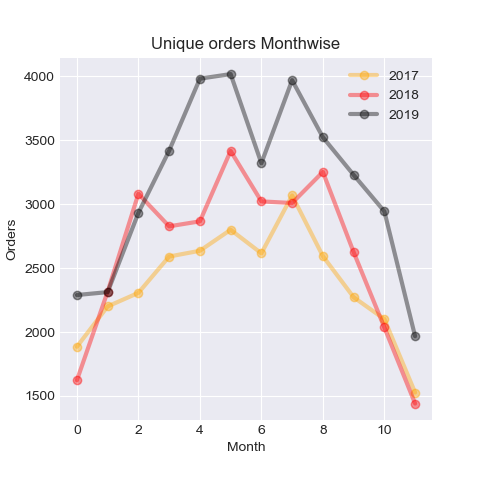
\includegraphics[scale=0.9]{chapters/figures/monthwise_orders.png}
    \caption{Trends in data-set.\\
    Source: Own Investigation}
    \label{fig:season}
\end{figure}
Another trend that is observed in the data-set is seasonality. The bike component industry is seasonal and is influenced by weather patterns. A similar trend of seasonality is also observed in the data-set. Fig \ref{fig:season} illustrates this buying trend in a two dimensional plot. The x-axis represent the months whereas the y-axis represent the number of orders. It is observed that the number orders increases consistently from the month of February (onset of spring season) and starts to decline from the month of July-August (onset of fall season). This pattern is clearly visible across all three years of data i.e. 2017,2018,2019 and highlights the fact that bike component industry is indeed influenced by the weather conditions.



\begin{figure}
    \centering
    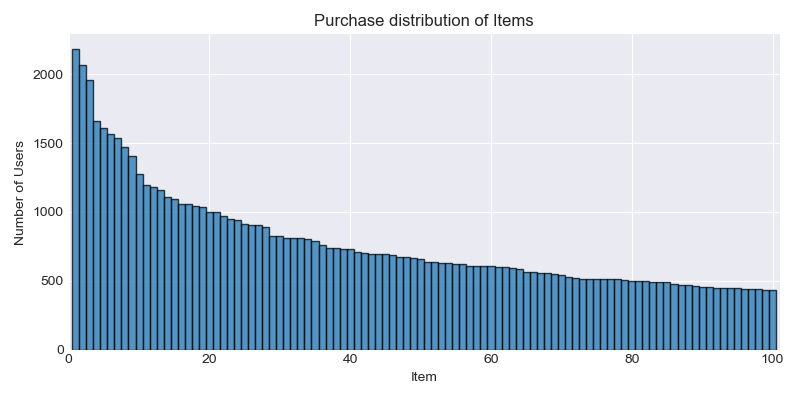
\includegraphics[scale=0.7]{chapters/figures/long_tail.png}
    \caption{Long tail plot.\\
    Source: Own Investigation}
    \label{fig:long_tail}
\end{figure}



\section{Machine Learning models}
This sub-chapter identifies different approach approach that are used to create a machine learning model for Context Aware Recommender System. Chapter 2 elaborates on the different types of Recommender System. Considering the theme of this work and the type of the data-set available, Collaborative Filtering based Recommender System is most suitable for this work. This is because of the unavailability of rich data about the users and the items. When the only source of data is explicit or implicit form, Collaborative Filtering methods are usually used. Collaborative Filtering methods identify the latent factors or hidden interest areas of the users, which can be utilized to recommended items matching the interest area. Collaborative Filtering methods can be divided into three categories namely: Nearest Neighbour, Latent Factor Model based, Hybrid (Nearest Neighbour + Latent Factor Model). Due to its efficiency in modelling users preferences, Model based approach is used for this work. \\
\Par

\begin{figure}
    \centering
    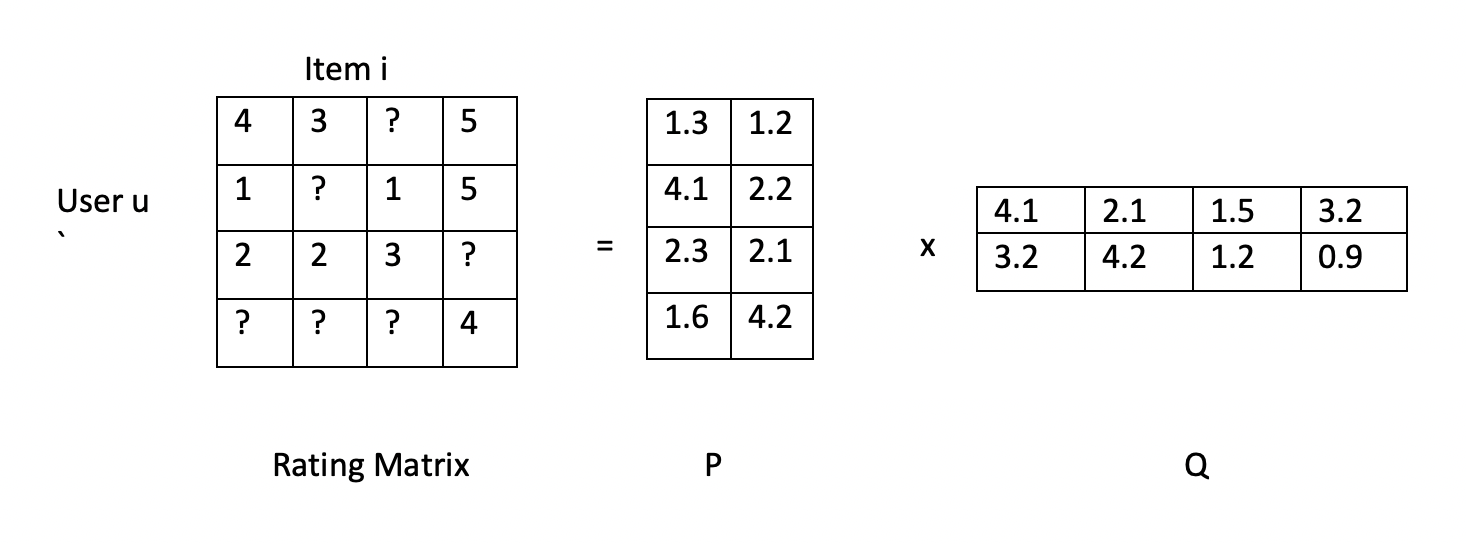
\includegraphics[scale=0.6]{chapters/figures/matrix_factorization.png}
    \caption{Decomposition of Rating Matrix into User Matrix P and Item Matrix Q.\\
    Source: Own Representation based on \textcite[44]{koren2009matrix}}
    \label{fig:matrix_factorization}
\end{figure}

The most common Latent Factor Model based approach for Collaborative filtering is Matrix Factorization. This technique is widely used while modelling a traditional recommender system based on the interactions between user-items. It is popular due to its scalability and higher predictive accuracy \autocite[43]{koren2009matrix}. As shown in Fig \ref{fig:matrix_factorization} the original user-item interaction matrix is decomposed into two different matrices \textit{P,Q} representing the users and the items respectively in \textit{k} dimension in other words different interest areas. Each entry in the decomposed matrices of user and item represents a vector of length \textit{k}. It is likely that the original user-item interaction matrix will be sparse and the missing ratings is denoted by ?. When the original matrix is decomposed,  the elements within these vectors represents a weight for each of the dimension. Thus when a dot product among these vectors result in an estimation of the rating for each interaction between the user and item \autocite[44]{koren2009matrix}. This estimate of the rating for an given user,item pair is represented by the Equation \ref{eqn:MF}. 

\begin{equation}
\label{eqn:MF}  r_u,_i = q_i^T.p_u
\end{equation}
where:
\begin{conditions}
 r_u,_i    &  estimated rating for user \textit{u, and item \textit{i}}.\\   
 q_i^T &  transpose of the item vector \textit{i} in \textit{P}. \\
 p_u & vector for user \textit{u} in \textit{Q} \\
\end{conditions}
\\
Since Matrix Factorization method handles both explicit and implicit data, this method is suitable for this study. Implicit feedback data is inferred from the users actions, thus resulting into less sparse user-item interaction matrix. The process of learning the latent factors in the matrices \textit{P,Q} involves minimizing the difference between the observed ratings in the user-item interaction matrix and estimated rating obtained using the Equation \ref{eqn:MF} the latent factors in matrices \textit{P,Q}. This estimation of a correct values of the latent factors is called as the learning process. This learning process is facilitated by a algorithms such as Stochastic Gradient Descent (SGD), Alternating Least Squares(ALS). For recommender systems dealing with implicit feedback data, ALS algorithm is preferred \autocite[45]{koren2009matrix}. This is because ALS algorithm is good in parallelizing, and the ability to handle implicit data while learning the parameters. \textcite[3]{Hu2008} proposed an adaptation to the Equation \ref{eqn:MF}, when working with implicit feedback data-sets and introduced an binary variable, preference \textit{c\textsubscript{u,i}} given by the Equation \ref{eqn:IMF}

\begin{equation}
\label{eqn:IMF}  p_{u,i}=\begin{Bmatrix}1   if r_{u,i} >0 \\0   if r_{u,i} =0 \end{Bmatrix} 
\end{equation}
where:
\begin{conditions}
 r_u,_i    &  estimated rating for user \textit{u} and \textit{item \textit{i}}.\\   
 p_u,_i & the confidence binary variable \\
\end{conditions}
\\
The estimated rating for user in cases of implicit feedback data-set is derived from counting the number of times a particular action was performed which in this scenario translates to the number of times a particular item was bought. A problem with implicit feedback is that it does not convey the exact emotion of the user action as only implication of the action can be drawn from it. For e.g. a product is bought with no intention of using. Thus to correctly measure the preference of the user \textcite[]{Hu2008} introduced confidence variable \textit{C\textsubscript{u,i}}. This confidence variable is calculated using the following equation
\ref{eqn:confidence}. This approach enables to have a confidence of estimating preference \textit{p \textsubscript{u,i}} =1.

\begin{equation}
\label{eqn:confidence}  c_{u,i}= 1 + \alpha * r_u,_i
\end{equation}
where:
\begin{conditions}
 r_u,_i    &  estimated rating for user \textit{u} and \textit{item \textit{i}}.\\   
 \alpha & the constant which control the rate of increase \\
\end{conditions}
\\

\Par
Matrix Factorization in a way represents a traditional recommender system where only the user-item interaction history is taken into consideration. There is no provision to integrate contextual information which represent the environment in which the user-item interaction takes place. Although subchapter 2.3 elaborates on the different methods of integrating contextual information i.e pre-filtering and post-filtering approach, they need constant fine tuning. A machine learning model based Context-Aware recommender system is more efficient and robust. There are many Machine learning model based approach which integrate contextual information. One such approach which works for explicit and implicit data is Factorization Machines. Factorization Machine extends the classic Matrix Factorization method by including additional contextual information. \textcite[3]{rendle2011fast}proposed this method which integrates the features which in this case can be contextual features for e.g. time, location and combine them together the user-item interaction to estimate the ratings for an item. An example of this is illustrated in fig \ref{fig:FM}. The data in this example is related to movie-recommendation system, where the Recommender Data (first entry) represents, the user A, interacts with item TI, has mood H (contextual feature), and watched with C (contextual feature) and rates the movie Ti 5 which is nothing but the target variable y.
This entry is represented in an binary format. Factorization Machines not only supports Categorical Features which in this example is represented by mood with values S,N,H but also supports numerical attributes \autocite[2]{rendle2011fast}. In this scenario, the rating is provided in the Target variable Y. During the training process the algorithm learns the pattern and tries to minimize the difference between the observed value of variable y and the estimated rating. This problem represents regression scenario. When rating data is not available for e.g. implicit data-set then the Target Variable Y takes binary values and the problem is classification where the prediction is either classified as 1 or 0. Similarly based on the example explained, this approach can be adapted to the data-set available for this study.  \\
\Par


Based on these observations, implicit Matrix Factorization and Factorization Machines based machine learning models can be used for this work since they provide the capability to analyze patterns within implicit data-set as well as contextual information. The following subchapter elaborates more on how these methods can be implemented and the architecture of the Recommender System. 

\Par
\begin{figure}
    \centering
    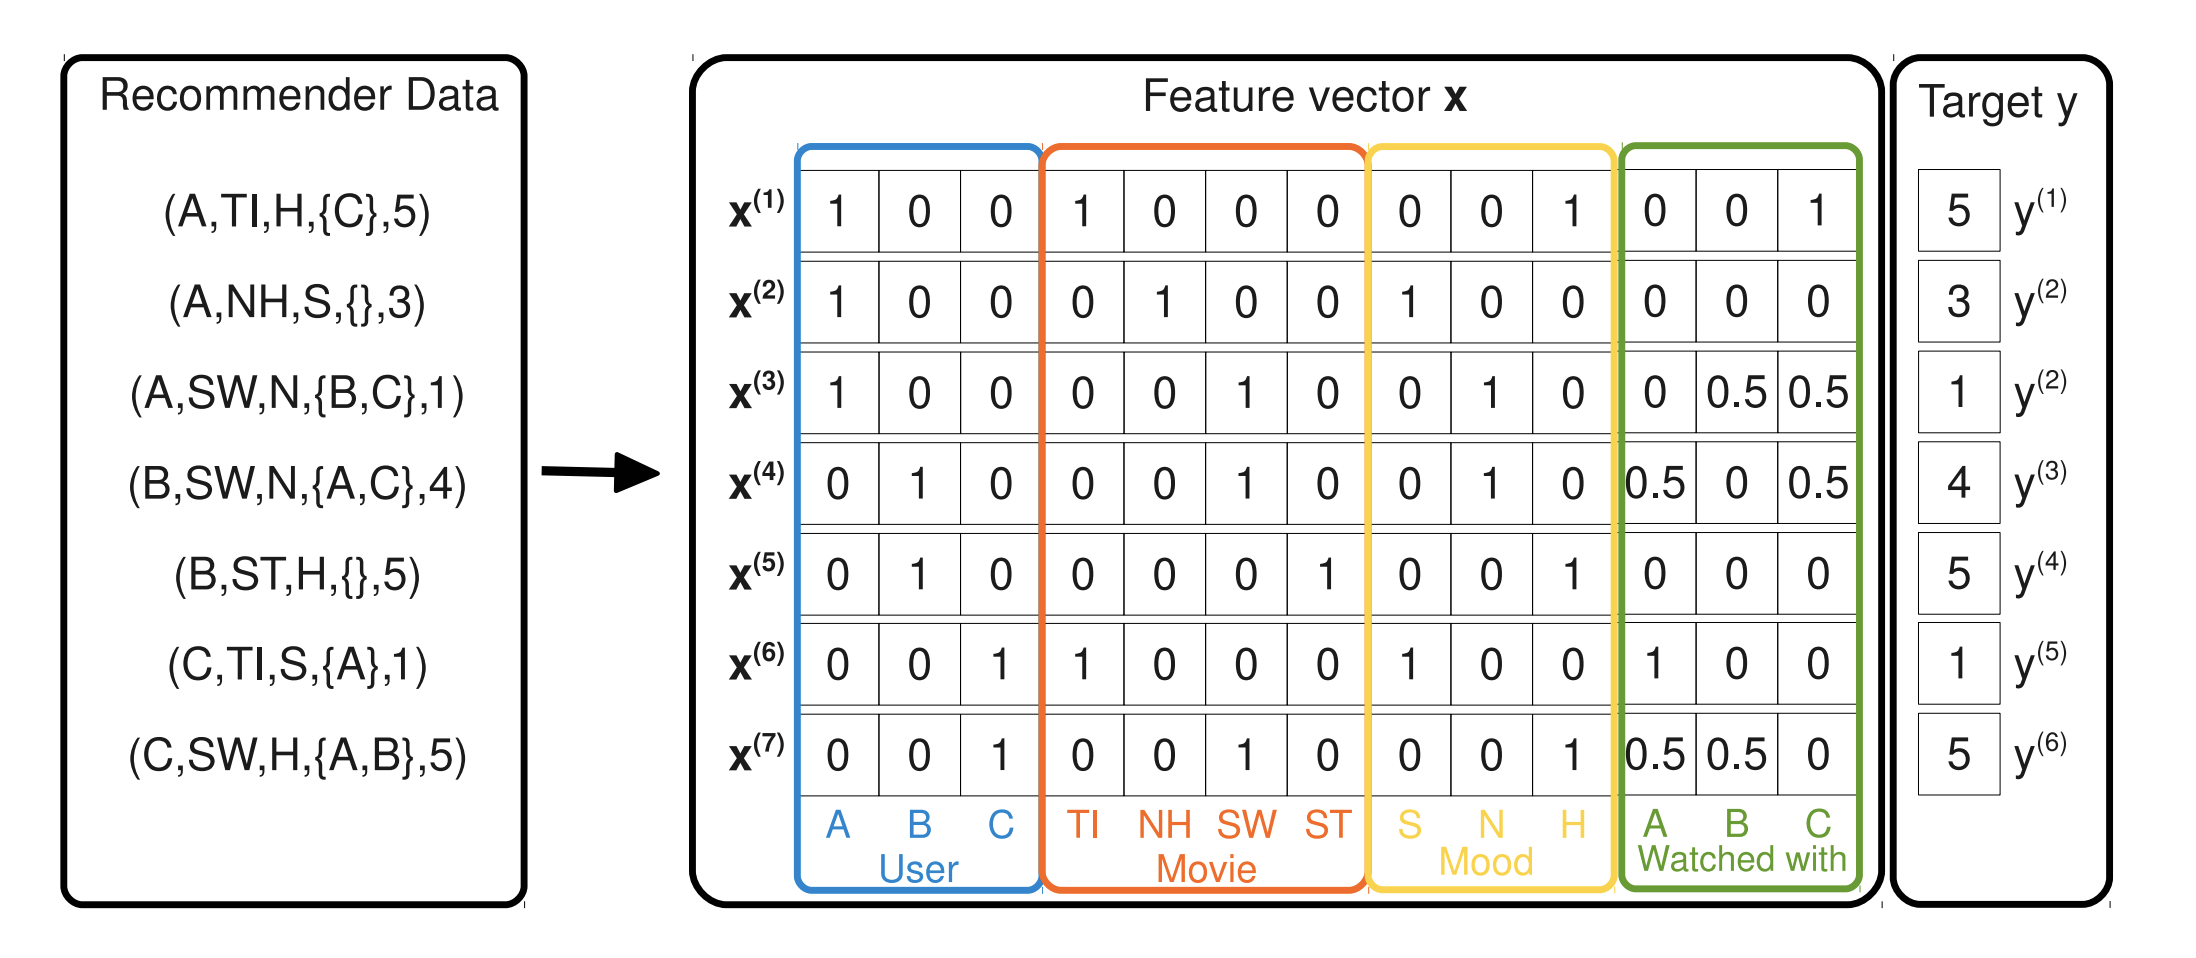
\includegraphics[scale=0.4]{chapters/figures/FM.png}
    \caption{Overview of the user-item interaction matrix along with the contextual features. \\
    Source: In \textcite[5]{rendle2011fast}}
    \label{fig:FM}
\end{figure}

\section{Implementation of Machine Learning models for Recommender System}
This step can be compared with the modelling step in the KDD process as discussed above. The use of Recommender System in the e-commerce industry is lucrative for companies considering the financial aspects related to it. Consequently many there has been a lot of research in this field, resulting in different approaches tailored for a specific scenario. Although most of the approach and algorithms developed are equipped to handle explicit data, there are not many algorithms that can handle both implicit, explicit data or only implicit data. Moreover, there are very few open source libraries which provide the implementation of the approach which can handle implicit data as well as contextual information while modelling a Context Aware Recommender System. Some of the example of such open source libraries are implicit\footnote[1
]{https://implicit.readthedocs.io/en/latest/index.html},lightFM \footnote[2]{https://making.lyst.com/lightfm/docs/index.html}, libFM \footnote[3]{http://libfm.org/}. \\

\Par
\begin{figure}
    \centering
    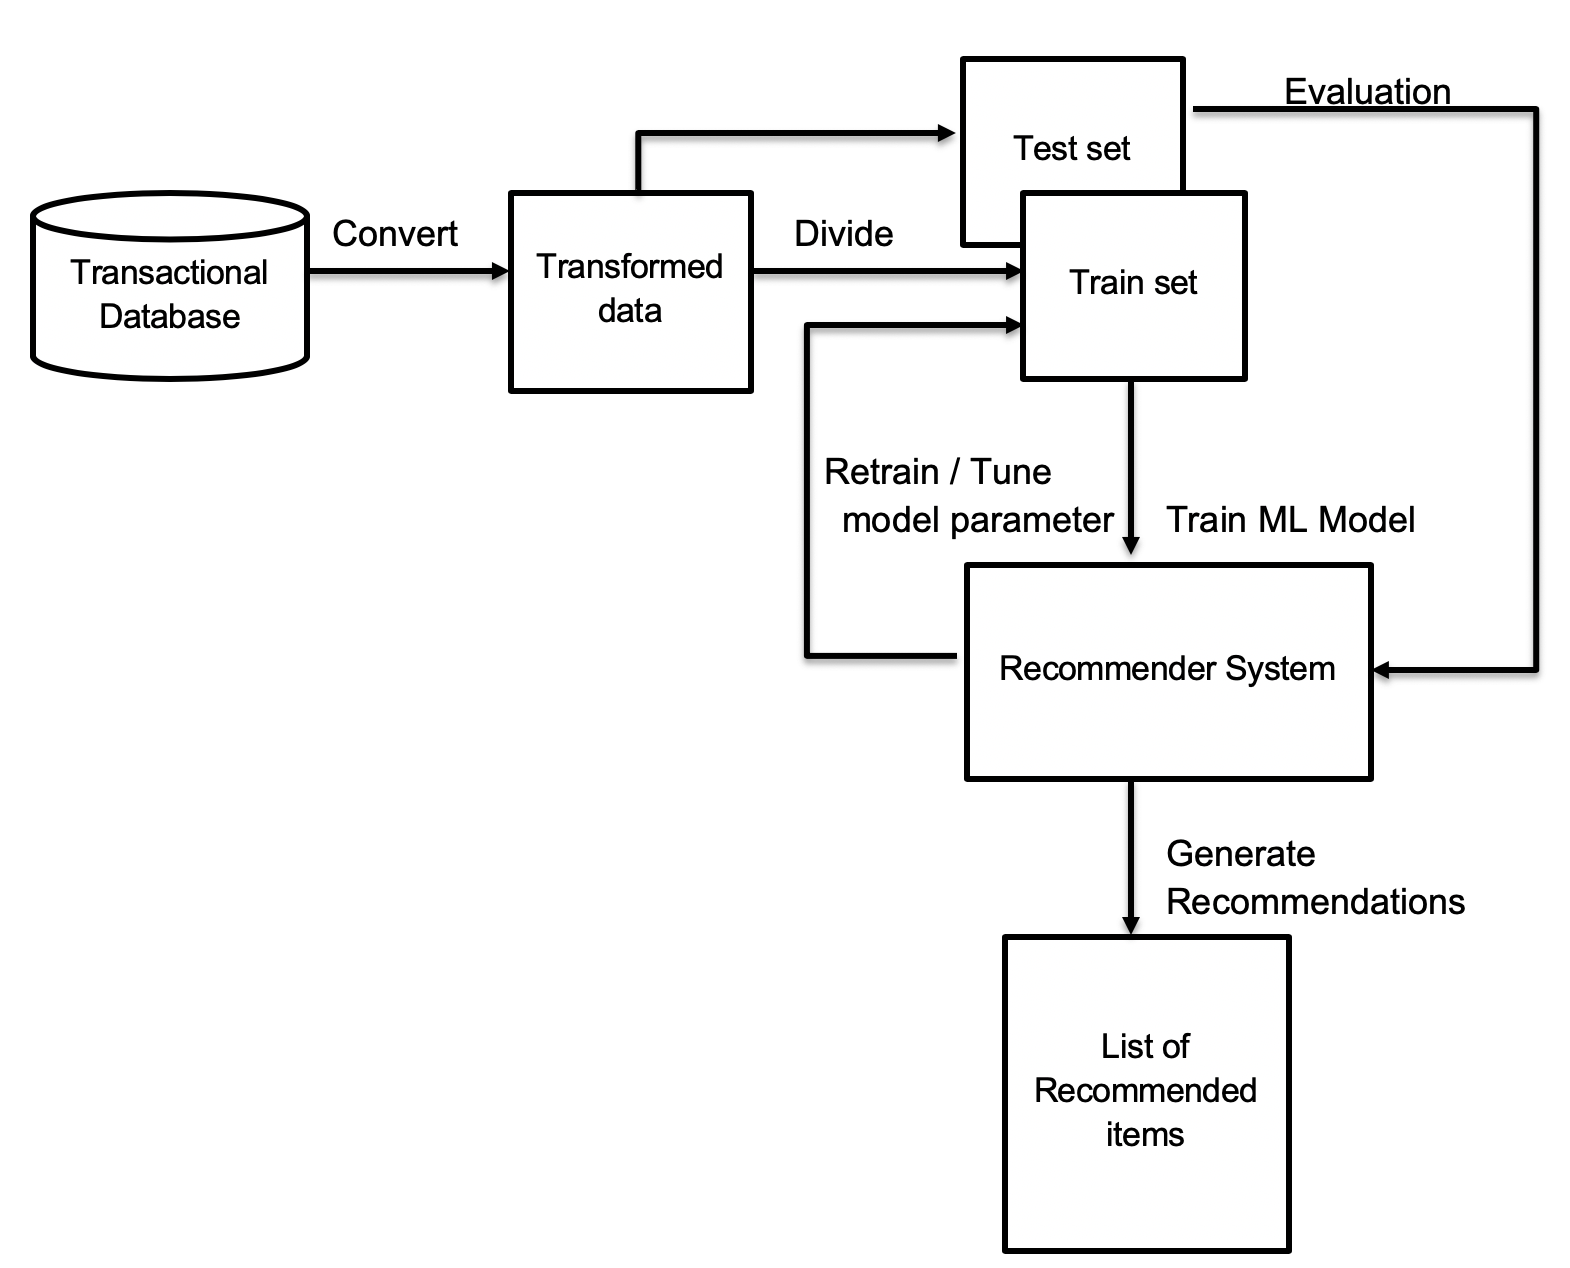
\includegraphics[scale=0.5]{chapters/figures/recommender_system.png}
    \caption{Recommender System process overview. \\
    Source: Own illustration}
    \label{fig:recommender_system}
\end{figure}

\\
\Par

Since this work is based on using the machine learning model based approach, the overview of the Recommender system  process is depicted in the Fig \ref{fig:recommender_system}. This also depicts the architecture of the system developed. The process follows the sequence of steps mentioned in the KDD phases in section \ref{sect:Kdd}, starting with the selection of the data-set from the transactional database, followed by pre-processing and transformation step which removes the anomalies and converts the transactional data present in the relational format into user-item matrix. This actually prepare the data in a format which the machine learning algorithm expects. Further to evaluate the performance of the machine learning algorithm, the data-set is converted into training and testing data-set. Unlike in any machine learning problem, formation of the training data-set and testing data-set is different in case of recommender system. A technique called as masking is used where certain percentage of the user-item interactions are masked to form the training data-set whereas the testing data-set is same as the original user-item interaction matrix. The training data-set is used to train the machine learning algorithm and evaluated on the testing data-set. The process of training the model is repeated until the desired performance is achieved. Furthermore the training data-set is used to identify the set of parameters also known as \textit{Hyper-parameters} specific to the algorithms. The process of finding the set of parameters which results in the desired performance level is known as \textit{Hyper-parameter tuning}. Depending on the type of the recommender system, different techniques are used to create the training and testing set. 
\\
\par
The main component of the Recommender System is the Machine Learning algorithm which learns different patterns within the training data-set. As discussed in the earlier sub chapter, matrix factorization and Factorization Based algorithms are suitable given the research theme of this work. Therefore, three different Machine Learning models are implemented which are evaluated and compared against the popularity baseline model. Evaluation metrics Mean Average Precision and Mean Average Recall are used to measure the performance. The models implemented described below:

\begin{itemize}
	\item \textit{Model 1: implicit ALS}\\
	This model represents the traditional Recommender System, which calculates the latent factors for both users and items using Alternating Least Squares algorithm. As the name suggests, the input data for this model is implicit in nature. Furthermore, no contextual information is included in the modelling process, thus it represents the traditional Recommender System.
	The training data is formatted into a user-item interaction matrix which is decomposed into user and item matrices using matrix factorization method. The estimated preference for the missing values in the sparse user-item matrix is calculated by using the Equation \ref{eqn:MF}.
	
	\item \textit{Model 2: LightFM}\\
	LightFM is Recommender System library which supports integrating user and item metadata and is designed to handle both implicit and explicit data-set. It is Hybrid Recommendation System which combines the power of content based recommendation system and collaborative filtering techniques. The advantage of using such Recommender System is that they can handle \textit{cold-start} problem, which is common in Recommender System \autocite[1]{kula2015metadata}. \textit{Cold-start} problem refers to a situation when there is no item interaction data about the new user, thus making it difficult to create a user profile and identify the user's preferences. Similarly for new items which have not interaction data with the users item profiles cannot be created. \\
	To train LightFM model the training data is represented in the user-item interaction matrix. Additionally, the information about the user is stacked together to create the user-feature matrix. Similarly item features are stacked to create the item-feature matrix. The estimated prediction for an user-item pair is calculated by using the following Equation 
	
	
    \begin{equation}
    \label{eqn:confidence}  r_u,_i =  f(q_u* p_i + b_u + b_i)  
    \end{equation}
    where:
    \begin{conditions}
     r_u,_i    &  estimated rating for user \textit{u} and \textit{item \textit{i}}.\\   
     q_u & the latent vector for user \textit{u}. \\ 
     p_i & the latent vector for user \textit{i}. \\ 
     b_u & the bias for user \textit{u} given by the sum of the bias of the user features. \\ 
     b_i & the bias for user \textit{i} given by the sum of the bias of the item features. \\
     f(x) & the sigmoid function given by  f(x)= 1 \div (1+ exp (-x)) \\
    \end{conditions}
    \\
	
	\item \textit{Model 3: libFM}\\
	libFM library implements the Factorization Machine method taking into consideration not only the user-item interactions but also the contextual data. The support of processing implicit as well explicit data makes it ideal to implement Context-Aware Recommender System. As shown in Fig \ref{fig:FM}, if the contextual information contains categorical information then they are encoded in a binary format to uniquely identify them. Numeric features for e.g. price can be included as it is and is not required to be encoded. The overall training data-set along with the contextual features is represented in a format shown below. 
	   
	   \textit{ Y <contextual{\_}feature1>: value1, <contextual{\_}feature2>:value2> ..... } \\
	   The observed rating or the implicit value i.e. bought or not/ clicked or not clicked represents the Y vector.
	
\end{itemize}
%%Although there are different techniques to generate recommendations, the Machine Learning based method %%are widely preferred. Machine Learning based models have proved to perform better in identifying the %%preferences of the users. For this reason

The completion of the training phase initiates the evaluation of the learned patterns on the test-set. Evaluation metric value is measured to judge the performance of the trained model. Furthermore, each model discussed above have set of parameters called as \textit{Hyper-parameters} which take certain values for the parameters defined. The process of finding the right parameter value to obtain the optimal performance is know as \textit{Hyper-parameter} tuning. \\
\Par
To support the implementation of the models discussed above, python programming language is suitable to support the easy manipulation of the data. Moreover, the libraries for theses models are implemented it python language which makes it more convenient to use.


%%\section{Result Interpretation}

